\documentclass[11pt,a4paper]{book}
\usepackage[utf8]{inputenc}
\usepackage[spanish]{babel}
\usepackage{amsmath}
\usepackage{amsfonts}
\usepackage{amssymb}
\usepackage{graphicx}

\usepackage[pdf]{pstricks}
\usepackage{pst-node,pst-circ,pst-plot,pst-3dplot,pst-all}

\author{Prof. Juan Manuel Maffei}
\title{Curso de mediciones eléctricas}
\begin{document}

	\newtheorem{ejemplo}{Ejemplo}[chapter]
	\tableofcontents
	\chapter{Sobre las mediciones}
\section{Magnitudes}
Medir es \textbf{comparar el valor de una magnitud con otro}, al que se consideró \textbf{la unidad} de dicha magnitud, a través de un experimento físico.

Una \textbf{magnitud} es toda aquella propiedad de un cuerpo que pueda ser medida.

La \textbf{cantidad} es el valor numérico que toma la medida dentro de un sistema de mediciones.

La \textbf{unidad} es la cantidad física que se toma como referencia para hacer las mediciones

\begin{ejemplo}
	Dada la expresión: Altura del edificio = 80 metros,
	\begin{itemize}
		\item Altura es la magnitud.
		\item 80 es la cantidad.
		\item metro es la unidad.
	\end{itemize}
	
	Quiere decir que la altura del edificio (magnitud: longitud) es 80 veces (cantidad) la longitud de referencia denominada metro (unidad).
\end{ejemplo}

Las unidades se fijan según acuerdos internacionales por el Comité Internacional de Pesos y Medidas. Recientemente, en noviembre de 2018, se votó la redefinición de algunas de las unidades fundamentales, incluida el Ampere (para medir corriente eléctrica).

Durante este curso, usaremos el \textbf{Sistema Internacional de Unidades}, pero es posible que en otros contextos se utilicen otros, como el sistema inglés o el CGS.
\subsection{Precisión y exactitud}
	Es común utilizar los términos \textbf{precisión} y \textbf{exactitud} como sinónimos, pero en el ámbito de la metrología, existe una diferencia:
	\begin{itemize}
		\item Precisión se refiere al grado de dispersión del conjunto de valores obtenidos en la medición repetida de una magnitud.
		\item Exactitud se refiere al grado de concordancia entre lo medido y su valor verdadero.
	\end{itemize}
\section{Sistema Internacional de Unidades}
\subsection{Unidades}

\begin{tabular}{|c|c|}
\hline 
Magnitud (símbolo) & Unidad (símbolo) \\ 
\hline 
longitud (L) & metro (m) \\ 
\hline 
masa (M) & kilogramo (kg) \\ 
\hline 
tiempo (T) & segundo (s) \\ 
\hline 
corriente eléctrica (I) & ampere (A) \\ 
\hline 
temperatura ($ \Theta $) & kelvin (K) \\ 
\hline 
intensidad lumínica (J) & candela (cd) \\ 
\hline 
energía (E) & julio (J) \\ 
\hline 
fuerza (F) & newton (N) \\ 
\hline 
potencia (P) & vatio (W) \\ 
\hline 
carga eléctrica (Q) & coulomb (C) \\ 
\hline 
tensión eléctrica, diferencia de potencial (V) & voltio (V) \\ 
\hline 
capacitancia & faradio (F) \\ 
\hline 
resistencia eléctrica (R) & ohmio ($ \Omega $) \\ 
\hline 
flujo magnético & weber (Wb) \\ 
\hline 
campo magnético & tesla (T) \\ 
\hline 
inductancia (L) & henrio (H) \\ 
\hline 
flujo luminoso & lumen (lm) \\ 
\hline
frecuencia & hertz (Hz) \\ 
\hline
\end{tabular} 

\subsection{Prefijos}\label{section:prefijos}

\begin{tabular}{|c|c|c|}
\hline 
Factor de multiplicación & Nombre  & Sı́mbolo  \\
\hline 
$10^{24}$                    & yotta   & Y       \\
$10 ^{21}$                    & zetta   & Z       \\
$10 ^{18}$                    & exa     & E       \\
$10 ^{15}$                    & peta    & P       \\
$10 ^{12}$                    & tera    & T       \\
$10 ^{9}$                     & giga    & G       \\
$10 ^{6}$                     & mega    & M       \\
$10 ^{3}$                     & kilo    & k       \\
$10 ^{2}$                     & hecto ∗ & h       \\
$10 ^{1}$                     & deka ∗  & da      \\
$10 ^{-1}$                    & deci ∗  & d       \\
$10 ^{-2}$                    & centi ∗ & c       \\
$10 ^{-3}$                    & mili    & m       \\
$10 ^{-6}$                    & micro   & $\mu $       \\
$10 ^{-9}$                    & nano    & n       \\
$10 ^{-12}$                   & pico    & p       \\
$10 ^{-15}$                   & femto   & f       \\
$10 ^{-18}$                   & atto    & a       \\
$10 ^{-21}$                   & zepto   & z       \\
$10 ^{-24}$                   & yocto   & y \\ \hline 
\end{tabular}

\subsection{Reglas}
\begin{enumerate}
	\item Los sı́mbolos son siempre impresos en letra tipo romana, indistintamente del tipo de letra usado en el resto del texto.
	\item Los sı́mbolos son escritos en minúscula excepto cuando el nombre de la unidad se deriva de un nombre propio.
	\item Los sı́mbolos de los prefijos se imprimen en letra tipo romana sin espacio entre los sı́mbolos del prefijo y la unidad.
	\item Los sı́mbolos nunca se pluralizan.
	\item Nunca use un punto después de un sı́mbolo, excepto cuando el sı́mbolo ocurre al final de una oración.
	\item Siempre use un espacio entre el número y el sı́mbolo, excepto cuando el primer caracter de un símbolo no es una letra.
	\item Los sı́mbolos se usan en conjunto con números en lugar de escribir el nombre completo de la unidad; cuando no hay números, las unidades se escriben con su nombre propio.
	
\end{enumerate}
\section{Consideraciones para la lectura de mediciones}
\subsection{Cifras significativas}
Según el nivel de precisión que se requiera en una medición, será necesario utilizar una determinada cantidad de cifras significativas.

Existen magnitudes continuas, que son aquellas que entre dos valores poseen infinitas posibilidades, y magnitudes discretas, que entre dos valores cualesquiera poseen una cantidad numerable y finita de posibilidades.

\begin{ejemplo}
	\begin{itemize}
		\item La cantidad de conductores dentro de una caja es una magnitud discreta (puede haber uno, dos, diez o incluso ningún cable, pero no 1,3 cables).
		\item La longitud de un conductor es una magnitud continua (puede medir 0,5 m, o 0,554 m, o 0,5533223 m).
	\end{itemize}
\end{ejemplo}

Las mediciones de magnitudes continuas siempre serán aproximadas, y las mediciones de magnitudes discretas, en muchos casos, pueden ser exactas.

El número de cifras significativas determinan la precisión de una medición.

Siempre que se opere con dos medidas, la precisión de ambas deberá ser consistente. Esto significa que si se suma una medición con precisión de decimales con otra con precisión de milésimos, el resultado será impreciso. En estos casos, el número con menor precisión determinará la precisión de la solución.
\subsection{Redondeo}
En muchos casos, será necesario redondear las mediciones. Para ello, se toma la lectura hasta el último dígito significativo que se esté considerando, sumando 1 al mismo si el próximo dígito es mayor o igual que 5, o dejándolo como está (truncar) si el próximo dígito es menor que 5.

\begin{ejemplo}
Si $V_1=3,25 V$, $V_2=2,4201 V$ y $V_3=3,245V$, 
	\begin{itemize}
		\item $V_1+V_2=3,25 V + 2,4201 V=5,6501 V=5,65 V$
		\item $V_1+V_3=3,25 V + 3,245 V = 6,495 V $. Como el número con menor precisión tiene dos dígitos decimales, deberá redondearse, sumando una unidad a las centésimas (porque el dígito de las milésimas es 5) obteniendo $6,50 V$ o $6,5V$.
	\end{itemize}
\end{ejemplo}
\subsection{Notación científica y de ingeniería}
En la sección \ref{section:prefijos}, se han usado, como factores de multiplicación, potencias de 10.

A veces, cuando los valores con los que se trabaja son muy grandes o muy pequeños, suele ser cómodo utilizar potencias de 10. De ese modo, puede expresarse estos valores indicando sólo sus cifras significativas, multiplicadas por una potencia de 10.

Si la potencia es positiva, el factor de multiplicación será un 1 y tantos ceros como indique el exponente:

\begin{tabular}{|c|c|c|}
\hline 
Valor & Potencia & Operación \\ 
\hline 
$1$ & $10^0$ & $10/10$ \\ 
\hline 
$10$ & $10^1$ & $10$ \\ 
\hline 
$100$ & $10^2$ & $10 \times 10$ \\ 
\hline 
$1000$ & $10^3$ & $10 \times 10 \times 10$ \\ 
\hline 
... & ... & ... \\ 
\hline 
1 y $n$ ceros & $10^n$ & $10 \times 10 \times 10 ... n$ veces \\ 
\hline 
\end{tabular} 

Si la potencia es negativa, debe recordarse la siguiente propiedad de las potencias:

$$ \frac{1}{10^{n}=10^{-n}} $$

Esto da lugar al siguiente razonamiento:

\begin{tabular}{|c|c|c|}
\hline 
Valor & Potencia & Operación \\ 
\hline 
$0,1$ & $10^{-1}$ & $1/10$ \\ 
\hline 
$0,01$ & $10^{-2}$ & $1/100$ \\ 
\hline 
$0,001$ & $10^{-3}$ & $1/1000$ \\ 
\hline 
$0,0001$ & $10^{-4}$ & $1/10000$ \\ 
\hline 
... & ... & ... \\ 
\hline 
$0,(n-1)$ ceros y $1$ & $10^{-n}$ & $1/1(n$ ceros $)$ \\ 
\hline 
\end{tabular}

\begin{ejemplo}
	\begin{itemize}
		\item $ 3 \times 10^{-3}=3\times \frac{1}{1000}=3\times 0,001 = 0,003 $
		\item $ 12 \times 10^{4}= 12 \times 1000 = 12000 $
		\item $ 3,25 \times 10^{6} = 3,25 \times 1000000 = 3250000 $
		\item $ 3,25 \times 10^{-4}= 3,25 \times 0,0001 = 0,000325 $
	\end{itemize}
\end{ejemplo}

En los ejemplos anteriores, se procedió a multiplicar un número por una potencia de 10, para obtener valores más pequeños o más grandes, y a simple vista resulta más legible.

Es una convención en notación científica, que la mantisa o coeficiente por el cual se multiplique la potencia de 10, debe estar entre 1 y 10.

La notación de ingeniería es similar, excepto que los exponentes de la potencia de 10 deben ser múltiplos de 3 y la mantisa debe estar entre 1 y 1000. Esto permite utilizar prefijos de magnitud como los que se enunciaron en la sección \ref{section:prefijos}.

\begin{ejemplo}
	\begin{itemize}
	Convertir las siguientes medidas para eliminar los prefijos, según la tabla de la sección \ref{section:prefijos}.
		\item $ 3 \mu F = 3\times 10^{-6} F=0,000003 F$
		\item $ 1,2 mA = 1,2 \times 10^{-3} A= 0,0012 A$
		\item $ 120 pF = 120 \times 10^{-12} F=0,000000000120 F$
		\item $ 22 M\Omega = 22 \times 10^{6} \Omega = 22000000 \Omega $
	\end{itemize}
\end{ejemplo}

\section{Mediciones directas e indirectas}

Una medición directa es la que se realiza con un instrumento sobre un determinado elemento, mientras que una medición indirecta involucrará, además, algún paso adicional mediante el cálculo.
\begin{ejemplo}
	
	\begin{itemize}
		\item Medir la tensión de un tomacorriente con un voltímetro es una medición directa.
		\item Con un voltímetro se mide la tensión en una rama de un circuito de CC. Luego se mide la corriente con un amperímetro en serie. Finalmente, se multiplican ambos resultados y con ello se obtiene la medición indirecta de la potencia.
	\end{itemize}		
\section{Generalidades de instrumentos de medición eléctrica}

\subsection{Instrumentos analógicos}

Los instrumentos de medición analógicos utilizan una aguja para visualizar las lecturas mediante una aguja, que se mueve de manera continua, al igual que la magnitud que se intenta medir.

En muchos casos, no requieren de alimentación externa, se visualiza de forma más sencilla la variación (crecimiento o decrecimiento) y no son muy sofisticados. 

Por otra parte, son más tendenciosos a errores de lectura groseros (por las confusiones en cuanto a las escalas), y tienen poca resolución.

Los instrumentos de medición analógica poseen un \textbf{alcance}, que es el valor máximo que puede medir dicho instrumento y una cantidad de divisiones denominadas \textbf{deflexiones}, que serán las que indiquen el valor medido según la posición de la aguja.

A partir de estas medidas, puede calcularse la \textbf{constante de lectura K}, que es la relación entre el alcance y la máxima cantidad de deflexiones. Esta medida indica la mínima unidad de variación legible.
$$ K = \frac{Alcance}{\alpha MAX} $$

El \textbf{rango de medida} es el tramo de la escala en el cual las lecturas son confiables mientras que el \textbf{rango de indicación} corresponde a toda la escala del instrumento.

\subsection{Instrumentos digitales}
	
Los instrumentos digitales muestran un número de varias cifras en vez de una escala continua. Lo hacen mediante un display digital de varios dígitos, y a veces con alertas sonoras o lumínicas.

Si bien su construcción es más compleja que la de los instrumentos analógicos y requieren una alimentación externa en todos los casos, tienen una alta resolución, evitan los errores de lectura, modifican muy poco el circuito en el que se conectan (impedancia de entrada muy alta) y son muy rápidos.

En algunos casos, se incluye la selección automática de escalas y permiten introducir sus datos directamente en otro sistema (computadoras) para poder procesarlos.

Los instrumentos digitales poseen una determinada \textbf{cantidad de dígitos}, que pueden ir de 0 a 9 y un \textbf{dígito de sobrerrango}, que sólo puede mostrar 0 ó 1.

La \textbf{sensibilidad}, en un instrumento digital, corresponde a el dígito menos significativo del rango.

La \textbf{resolución}, por otra parte, no tiene unidad. Para calcularla, se debe pensar en la máxima lectura posible y dividir el valor mínimo que puede medir el último dígito sobre esta lectura máxima.

$$ \textit{Resolución} = \frac{1}{10^{d}} \textit{siendo $d$ la cantidad de dígitos}$$

La resolución también se suele expresar como porcentaje.

Con estos datos, se puede hallar la sensibilidad en función de la resolución del instrumento:
$$ Sensibilidad = \frac{\textit{Resolución x Valor a plena escala}}{100} $$
\end{ejemplo}	
	
\chapter{Errores}

Holaaaa
	\chapter{Magnitudes eléctricas}

En este capítulo, arribaremos a definir \textbf{intensidad de corriente eléctrica}, \textbf{tensión eléctrica}, \textbf{resistencia eléctrica}, y veremos cómo estas tres magnitudes se encuentran relacionadas. Para ello, será necesario contar con nociones acerca de los átomos y su estructura. Tranquilo... no nos detendremos demasiado en estas ideas, pero debés saber que son fundamentales para poder construir una base sólida en la comprensión de los fenómenos eléctricos.

\section{El átomo}

La materia está constituida por unidades muy pequeñas (del orden de los picómetros) llamadas \textbf{átomos}.

Para tener una noción más clara de la pequeñez de los átomos, \textit{el diámetro de un átomo es al diámetro de una manzana como el diámetro de una manzana es al diámetro de la Tierra}.

A su vez, estos átomos poseen un \textbf{núcleo}, formado por \textbf{protones} y \textbf{neutrones}, y uno o varios \textbf{electrones}; todos atraídos o repelidos por lo que se conoce con el nombre de \textbf{fuerza eléctrica}.

Imaginemos por un segundo que en el Universo, todas las partículas se atrayeran entre sí... Toda la materia estaría comprimida en un único bloque compacto.

Si, por el contrario, todas las partículas se repelieran, el Universo sería un gas en permanente expansión.

Es lógico pensar entonces, que estos tres tipos de partículas (protones, neutrones y electrones), se encuentren atraídas o repelidas entre sí de manera equilibrada para que el Universo pueda subsistir tal y como lo conocemos.

Se dice que los protones tienen carga eléctrica positiva, que repele cargas positivas pero que atrae cargas negativas. Entonces, estos protones positivos en el núcleo, atraen a una nube de electrones negativos a su alrededor para constituir el átomo.

Los electrones, con carga negativa, son atraídos por el núcleo positivo de protones, pero se rechazan entre sí. Son muy ligeros y se mueven muy rápido. 

Debido a este rechazo entre los electrones, no atravesamos una pared al tocarla, ya que los electrones de nuestra mano rechazan a los electrones de la pared.

Si bien la masa de un protón es mucho mayor a la de un electrón, ambos poseen la misma cantidad de carga eléctrica (es decir que un electrón es tan negativo como positivo es un protón). 

Las fuerzas eléctricas de atracción y repulsión, harán que las cargas de un átomo se encuentren balanceadas. En otras palabras: un átomo tendrá la misma cantidad de protones que de electrones, y entonces es eléctricamente neutro.

Aunque los átomos tengan carga neutra, es posible que los electrones de sus capas externas, sean atraídos por el núcleo de otros átomos, provocando una ``asociación" que da lugar a la formación de moléculas.

\subsection{Fuerza eléctrica}

Según la cantidad de electrones que se encuentren atraídos al núcleo de un átomo, se organizarán en diferentes capas o niveles de energía. Mientras la distancia al núcleo sea mayor, la \textbf{fuerza eléctrica} será menor.

La fuerza eléctrica es una magnitud vectorial, que aparece entre dos cuerpos cargados eléctricamente, y puede ser de atracción o de repulsión.

Para comprender mejor la fuerza eléctrica, podemos recurrir a una analogía con la fuerza magnética, con la que hemos experimentado toda la vida: 
A medida que acercamos un imán fijo a un metal, podemos percibir que la fuerza de atracción entre ambas piezas es mayor, y a medida que lo alejamos, la fuerza es menor.

La fuerza eléctrica entre dos cuerpos cargados se calcula mediante la Ley de Coulomb:

$$ F = k \times \frac{q_1 \times q_2}{d^{2}} $$

\begin{itemize}
	\item $k=9 \times 10^{9}\frac{N.m^{2}}{C^{2}}$
	\item $q_1$ y $q_2$ son las cantidades de carga de ambos cuerpos, expresados en Coulombs.
	\item $d$ es la distancia que separa ambos cuerpos.
\end{itemize}

Con respecto a la unidad de carga, \textit{1 Coulomb} equivale a aproximadamente $6,241509\times 10^{18}$ electrones, o $6,24$ millones de billones de electrones... que si bien es una cantidad enorme, sólo representa a la carga que pasa por un cargador de teléfono celular durante unos pocos segundos.

\subsection{Materiales conductores y aislantes}

Aplicando esta Ley, puede deducirse que los electrones de un átomo pueden estar fuerte o débilmente atraídos por el núcleo según la distancia que mantengan con respecto al núcleo.

Si la atracción entre el núcleo y alguno de sus electrones es débil, ese material es conductor. Si, por el contrario, todos los electrones del átomo se encuentran fuertemente atraídos por el núcleo, no se podrán desprender con facilidad del átomo y por lo tanto son materiales aislantes.

Pero la atracción de los electrones con los núcleos de sus respectivos átomos no depende sólo de su ``cercanía al núcleo" sino también de la completud de las capas: los átomos con capas completas suelen ser estables y los átomos con capas incompletas suelen tener más facilidad para ceder electrones (recordando que un material que cede electrones con facilidad es un conductor).

Una capa de electrones puede contener hasta $2n^{2}$ electrones, donde $n$ es el número de capa.

Tomemos como ejemplo el cobre, cuyos átomos poseen 29 protones y 29 electrones.

Los electrones se encuentran distribuidos de la siguiente forma:
\begin{itemize}
	\item Capa 1: 2
	\item Capa 2: 8
	\item Capa 3: 18
	\item Capa 4: 1
\end{itemize}

El electrón de la cuarta capa, se encuentra alejado del núcleo, y además, está en una capa incompleta, porque la cuarta capa puede contener hasta $2\times 4^{2}=32$ electrones, y por estos motivos el cobre es buen conductor de corriente eléctrica.

Si hubiera, en las inmediaciones del átomo de cobre, una fuerza de atracción lo suficientemente fuerte, el electrón de la cuarta capa se liberaría del átomo padre, quedando el átomo con 29 protones y 28 electrones y carga positiva. Cuando esto ocurre, el átomo se convierte en un ion positivo.

\section{Diferencia de potencial eléctrico o tensión}

Algo similar ocurre en todas las baterías: una separación de cargas positivas y cargas negativas, a través de medios químicos.

Una fuente de tensión no es más que un dispositivo con regiones de carga positiva y carga negativa. Mientras mayores sean estas cargas, mayor será la tensión o voltaje.

Para efectuar este proceso de separación de cargas, es necesario gastar cierta energía. Así, la \textbf{diferencia de potencial} se define como el trabajo necesario para mover estas cargas.

\begin{equation} \label{eq:1}
  \text{Dif. de potencial eléctrico } \textbf{ V} = \frac{\text{energía potencial }\textbf{ W}}{\text{carga }\textbf{ Q}}
\end{equation}


Si utilizamos las unidades del S.I., se dice que \textit{1 Volt de potencial equivale a 1 Joule de de energía por 1 Coulomb de carga}

$$ 1 V = 1 \frac{J}{C} $$

\begin{ejemplo}
	Determinar la tensión entre dos puntos si se requieren 80 J de energía para mover 20 C de carga.
	
	\emph{Solución:} Aplicando la ecuación \ref{eq:1}, se tiene $$ \frac{80J}{20C}=4V $$.
\end{ejemplo}

\begin{ejemplo}
	Determinar la energía consumida para mover una carga de 0,05 C entre dos puntos si la tensión entre los mismos es de 10 V.
	
	\emph{Solución:} De la ecuación \ref{eq:1}, se despeja $$ \text{Energía potencial} = \text{Potencial eléctrico} \times \text{carga} $$
	
	Luego $$ 0,05C \times 10V = 0,5 J $$
\end{ejemplo}

\section{Intensidad de corriente eléctrica}

La corriente eléctrica o intensidad de corriente eléctrica, es el flujo de cargas eléctricas; es decir, el movimiento de electrones a lo largo del tiempo.

\begin{equation}
\label{eq:2}
	I=\frac{Q}{t}
\end{equation}

La unidad que utilizamos para la corriente es el Ampere, y equivale a 1 Coulomb de carga fluyendo durante 1 segundo de tiempo:

$$ 1A = \frac{1C}{1s} $$

\begin{ejemplo}
	Determinar la corriente eléctrica en Amperes si la carga que fluye es de 0,01 C durante 5 mS.
	
	\emph{Solución:} De la ecuación \ref{eq:2} se sabe que las unidades deberán ser Coulomb para las cargas y segundos para el tiempo. Por ello, debe realizarse la conversión $5mS=\frac{5}{1000} S =0,005 S$, y a continuación, aplicar la ecuación, obteniendo: $$ I= \frac{0,01 C}{0,005 S} = 2 A $$
\end{ejemplo}

\begin{ejemplo}
	Calcular cuánto tiempo deberá pasar para que circule 1 C de carga si la corriente en un circuito es de 0,3 A.
	
	\emph{Solución:} De la ecuación \ref{eq:2} se despeja el tiempo, obteniendo: 
	\begin{equation}
		\label{eq:3}
		t=\frac{Q}{I}
	\end{equation}
	Y luego, es inmediato que $$ t=\frac{1C}{0,3A}=(1/3)S \approx 0,333 S $$
\end{ejemplo}

\section{Relación entre tensión y corriente: la resistencia}

Es común confundir tensión con corriente, pero son dos términos completamente diferentes.

Aplicar una tensión a un material conductor hará que fluya corriente eléctrica por el mismo.

La tensión es la causa, mientras que la corriente es la consecuencia.

Sin tensión no puede haber corriente eléctrica, pero sí puede existir tensión entre dos puntos sin una corriente que circule entre los mismos (esto ocurre, por ejemplo, entre los bornes de una pila que no está conectada en un circuito, ya que existe tensión pero no hay corriente circulando entre los mismos).

Si la tensión es la causa de la corriente, evidentemente una modificación de los valores de tensión alterará la corriente obtenida.

La \textbf{resistencia} es la medida de la oposición que presenta un determinado material al paso de la corriente eléctrica. Para medirla, se utiliza como unidad el \textbf{Ohmio}, que se simboliza con la letra griega $\Omega$ .
\subsection{Ley de Ohm}
Si se piensa en una definición del tipo $ \textit{Efecto} = \frac{\textit{Causa}}{\textit{Oposición}}$, se puede definir la \textbf{Ley de Ohm} como sigue:

\begin{equation}
	\label{eq:ohm_i}
	I=\frac{V}{R}
\end{equation}
donde $V$ es la tensión en Voltios, $I$ es la intensidad de corriente en Amperes y $R$ es la resistencia en ohmios.

\begin{figure}[h]
	\label{gr:ohm}
	\caption{Circuito básico}
	
%	\begin{pspicture}(0,0)(6,5)
%
%		\pnodes(1,1){A}(1,4){B}(5,1){C}(5,4){D}
%		\vdc(B)(A){$V$}
%		\resistor[dipolestyle=zigzag, tensionlabel=$I$](C)(D){$R$}
%
%		\wire(A)(C)
%		\wire(B)(D)
%	\end{pspicture}

\end{figure}

De la ecuación \ref{eq:ohm_i} se pueden despejar:
\begin{equation}
	\label{eq:ohm_v}
	V=I \times R
\end{equation}
\begin{equation}
	\label{eq:ohm_r}
	R=\frac{V}{I}
\end{equation}
\section{Potencia (para corriente continua)}
La \textbf{potencia} es la cantidad de trabajo que puede realizarse en una cantidad de tiempo. En otras palabras, es \textit{la velocidad a la que se realiza un trabajo}.

\begin{ejemplo}
	Un motor GRANDE posee más potencia que un motor PEQUEÑO porque puede realizar más trabajo en la misma cantidad de tiempo.
\end{ejemplo}

En términos analíticos, la potencia (en Watts o vatios) es la relación entre trabajo (en Joules) y tiempo (en segundos).

\begin{equation}
	\label{eq:pot}
	P = \frac{W}{t}
\end{equation}

Despejando $W$ en la ecuación \ref{eq:1}, se obtiene $ W=QV $. Esto puede aplicarse en la ecuación \ref{eq:pot}, obteniendo:

$$ P =\frac{QV}{t}=V\frac{Q}{t} $$

Finalmente, reemplazando la ecuación de corriente \ref{eq:2} en ésta última, se obtiene:
\begin{equation}
	\label{eq:pot_cc1}
	P = V \times I
\end{equation}

También puede reemplazarse esta última ecuación en la Ley de Ohm, obteniendo:

\begin{equation}
	\label{eq:pot_cc2}
	P = \frac{V^{2}}{R}
\end{equation}

\begin{equation}
	\label{eq:pot_cc3}
	P = I^{2}R
\end{equation}

\subsection{Energía}

Para que la potencia convierta energía de cualquier forma, se debe utilizar durante un tiempo. Cuanto más tiempo se consuma la potencia, mayor será la energía consumida.

\begin{equation}
	\label{eq:w}
	W=P\times t \text{ energía en Watts/hora}
\end{equation}

\begin{equation}
	\label{eq:w_kwh}
	W=P\times t \times 1/1000 \text{ energía en kiloWatts/hora}
\end{equation}
La energía $W$ se medirá en $Wh$ (watts/hora) o $kWh$ (kilowatts/hora) según convenga.

Nótese que la unidad para el tiempo establecida por el SI es el segundo, pero en este caso resulta muy pequeño (y por lo tanto los valores medidos usando esta unidad serían muy grandes), y debe tenerse especial cuidado al operar con estas magnitudes, ya que puede ser necesario realizar conversiones.

\subsection{Eficiencia}

La eficiencia $\eta$ (eta) se define como la relación entre la \textbf{potencia de entrada} y la \textbf{potencia de salida} del sistema.
\begin{equation}
	\label{eq:efi}
	\eta = \frac{P_{salida}}{P_{entrada}}
\end{equation}

Este es un valor decimal que varía entre 0 y 1. Habitualmente, se lo suele expresar en porcentaje (por lo que se debería multiplicar la expresión anterior por 100)

\begin{equation}
	\label{eq:efiporc}
	\eta \% = \frac{P_{salida}}{P_{entrada}} \times 100
\end{equation}

Si la eficiencia de un sistema fuera del 100$\%$, esto significaría que su potencia de entrada es igual a la potencia de entrada. En la práctica, sabemos que esto no es posible, porque todo sistema tendrá pérdidas por transformación de energía, y esto implica una diferencia entre las potencias: $$ P_{entrada} = P_{salida} + P_{perdida} $$ 

\section{Campos eléctricos}

Alrededor de un cuerpo cargado, existirá un \textbf{campo eléctrico}. A medida que la distancia al cuerpo sea menor, la \textbf{densidad del campo eléctrico} será mayor.

La \textbf{densidad de flujo } se define como la relación entre las líneas de flujo y el área que se está evaluando. Como la densidad de carga aumenta consecuentemente con la carga eléctrica, ambas magnitudes (carga y flujo) pueden igualarse. $$ \text{Densidad} = \frac{\text{Carga}}{\text{Área}} $$

La \textbf{fuerza del campo eléctrico} $F_{ce}$ es la fuerza que actúa sobre una carga Q en un punto:
$$ F_{ce} = \frac{F}{Q} $$

Reemplazando la fuerza en la ecuación anterior según la \textit{Ley de Coulomb}, se obtiene: 
\begin{equation}
	\label{eq:fuerza_electrica_capacitor}
	F_{ce} = \frac{kQ}{r^{2}}
\end{equation}


Esto quiere decir, que la fuerza del campo eléctrico está relacionada con el tamaño de la carga y la distancia que se mantenga con ésta. A medida que la distancia sea mayor, la fuerza eléctrica será \textit{mucho menor} (dado que el término en el denominador está elevado al cuadrado).

\subsection{Capacitores}

Existe un componente electrico cuyo principio de funcionamiento está directamente relacionado con los campos eléctricos: \textbf{el capacitor}.

\subsubsection{Construcción y principio de funcionamiento}

Un capacitor está constituido por dos placas conductoras paralelas separadas a una distancia mínima, por un material \textbf{dieléctrico} (aislante), que puede ser aire, mica, cerámica, poliéster, entre otros.

\begin{figure}[htbp]
  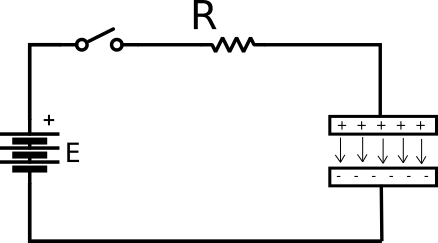
\includegraphics[scale=1]{images/capacitor_circuito_carga}
  \caption{Circuito de carga básico de un capacitor}
  \label{fig:cap_carga}
\end{figure}

Dado el circuito de la figura \ref{fig:cap_carga}, al cerrar el interruptor y por ahora omitiendo la resistencia (o suponiendo que posee una resistencia de $0 \Omega$), la placa inferior se comenzará a cargar con electrones libres, y la placa superior con cargas positivas.

Entre las placas, se alcanzará la tensión de la fuente $E$.

Como la distancia entre ambas es muy pequeña, las cargas se verán atraídas por una fuerza eléctrica (que recordando la ecuación \ref{eq:fuerza_electrica_capacitor}, será mayor si la distancia entre ambas es menor), y permanecerán atraídas incluso si se elimina la fuente de alimentación (o si se abre el circuito con el interruptor).

\begin{figure}[htbp]
  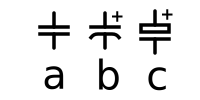
\includegraphics[scale=1]{images/capacitor_simbolo}
  \caption{Símbolos del capacitor: (a) No polarizado, (b) y (c) Polarizado}
  \label{fig:cap_simbolos}
\end{figure}

\subsubsection{Capacitancia}

La \textbf{capacitancia} de un capacitor es la cantidad de cargas que puede almacenar en él, cuando está completamente cargado.

\begin{equation}
	\label{eq:capacitancia}
	C = \frac{Q}{V}
\end{equation}

La unidad utilizada para medir la capacidad es el \textbf{Farad}, y 1 Farad de carga equivale a una carga de 1 Coulomb a una diferencia de potencial de 1 volt.
$$ 1 \text{Farad} = \frac{1 C}{1 V}$$

Redefiniendo la ecuación \ref{eq:fuerza_electrica_capacitor} para el caso del capacitor, resulta
\begin{equation}
	F_{ce} = \frac{V}{d}
\end{equation}

considerando la fuerza eléctrica en $Voltios/metro$, la tensión en $voltios$ y la distancia en $metros$.

El campo eléctrico también es afectado por la \textbf{permitividad} del material que se utiliza como dieléctrico. Un aumento en la permitividad del material, permitirá que la misma carga se almacene con un campo eléctrico menor; es decir, con un potencial eléctrico menor. Analizando la ecuación \ref{eq:capacitancia}, si la tensión disminuye, la capacitancia aumentará. En otras palabras, \textit{si la permitividad del dieléctrico es mayor, la capacidad será mayor}.

La permitividad $\epsilon $ se define como $ \epsilon = \frac{\epsilon_r}{\epsilon_0}$, donde $\epsilon_r$ es la permitividad relativa del material y $\epsilon_0 $ es la permitividad del vacío.

En la siguiente tabla, se recopilan los valores de algunos materiales utilizados para la construcción de dieléctricos de capacitores.

\begin{tabular}{|c|c|}
\hline 
Material & Permitividad relativa \\ 
\hline 
Aire & 1,0006 \\ 
\hline 
Papel & 1,5 \\ 
\hline 
Aceite & 2,8 \\ 
\hline 
Mica & 4 \\ 
\hline 
Cuarzo & 4,5 \\ 
\hline 
Baquelita & 5 \\ 
\hline 
PVC & 30 a 40 \\ 
\hline 
Agua destilada & 80 \\ 
\hline 
Acetona & 191 \\ 
\hline 
\end{tabular} 

Si se desea calcular la capacitancia teniendo en cuenta los valores de permitividad eléctrica, la ecuación es la siguiente,

\begin{equation}
	\label{eq:capacitancia_permitividad}
	C = \epsilon \frac{A}{d}
\end{equation}

considerando $\epsilon $ en $Farad/metro$, el área en metros cuadrados, la distancia en metros y la capacidad en Farads.

Debe tenerse en cuenta que los capacitores poseen un \textbf{voltaje de trabajo máximo}, que representa la máxima tensión que puede aplicarse en forma continua sin dañar el dispositivo. Si se excede, se puede dañar el dieléctrico.

\section{Campos magnéticos}
imán permanente, líneas de flujo magnético
densidad de flujo magnético
\subsection{Inductores}
\subsubsection{Construcción}
\subsubsection{Inductancia}
\subsubsection{Tensión inducida}
\subsubsection{Tipos de inductores}

	% Sistemas de puesta a tierra
	% Grados de electrificación
		% Potencia máxima, coeficiente de simultaneidad.
		% Mediciones de puesta a tierra
		% Resistencia de electrodos
	% Seguridad
	\chapter{Instrumentos de medición}

Incluir cómo afecta a las mediciones la variación de la Temperatura.
\section{Multímetro}
\subsection{Voltímetro}
\subsection{Amperímetro}
\subsection{Óhmetro}
\section{Vatímetro}
\section{Capacímetro}
\section{Frecuencímetro}
\section{Pinza amperométrica}
\section{Megóhmetro}
\section{Telurímetro}
\section{Osciloscopio}
\section{Comprobadores de tensión}
\subsection{Buscapolo}
\subsection{Medidor inductivo}
\section{Cofímetro}
\section{Medidor de energía}
\section{Medidor de campo electromagnético}	
	
	\begin{thebibliography}{X}
	% \bibitem{Ref2} \textsc{Autores}, (AÑO). \textit{Título}, ciudad, editorial.	
	\bibitem{boylestad} \textsc{Boylestad, R.}, (2011). \textit{Introducción al análisis de circuitos} Decimosegunda edición, México, Pearson Educación.
	\bibitem{hewitt} \textsc{Hewitt, P.} (2002). \textit{Conceptual physics}. Pearson Educación.
	\bibitem{bolton} \textsc{Bolton, W.} (1995). \textit{Mediciones y pruebas eléctricas y electrónicas}. Marcombo.
	\bibitem{uniandes} \textsc{Calderón, J.} (2006). \textit{Fundamentos de las Mediciones Eléctricas. Teorı́a y Prácticas de Laboratorio}. Escuela de Ingenierı́a Eléctrica, Universidad de Los Andes.
	\bibitem{utnmendoza} \textsc{Samsó, F.} (2008). \textit{Apuntes de Cátedra de Máquinas e Instalaciones Eléctricas}. Departamento de Electŕonica. Universidad Tecnológica Nacional: Facultad Regional Mendoza.
	\bibitem{maqelec} \textsc{Ortega, G.; Gómez, M. \& Bachiller, A.} (2002). \textit{Problemas Resueltos de Máquinas Eléctricas}. Thomson. Madrid.
	\bibitem{suarez} \textsc{Suárez, J. A.} (2006). \textit{Medidas Eléctricas: segunda edición}. Libro de cátedra de Mediciones Eléctricas I: Facultad de Ingeniería, Universidad Nacional de Mar del Plata.
	\bibitem{frank} \textsc{Frank, E.} (1969). \textit{Análisis de Medidas Eléctricas}. McGraw Hill. Madrid.
	\bibitem{aeabt} \textsc{Asociación Electrotécnica Argentina} (2007). \textit{Documento Normativo 95150. Suministro y medición en baja tensión}. AEA.
	\bibitem{aeamantenimiento} \textsc{Asociación Electrotécnica Argentina} (2006). \textit{Documento Normativo 90706 Guía para la gestión del Mantenimiento en instalaciones. }. AEA.
	\bibitem{aeamantenimiento} \textsc{Asociación Electrotécnica Argentina} (2006). \textit{Documento Normativo 90364-7-771 Reglamentación para la ejecución de instalaciones eléctricas en inmuebles – Viviendas, oficinas y locales (unitarios). }. AEA.
	%Materiales del curso de EDx
	
\end{thebibliography}
\end{document}